%
%

\begin{tikzpicture}[scale=\figurewidth]
    \tikzstyle{image} = [inner sep=0, outer sep=0, node distance = 0 and 0]
    \pgfplotsset{colormap={warm}{
    rgb=(1, 1, 1)
    rgb=(0.98823499999999997, 0.98039200000000004, 0.87058800000000003)
    rgb=(0.99215699999999996, 0.96470599999999995, 0.71372500000000005)
    rgb=(0.98823499999999997, 0.95686300000000002, 0.64313699999999996)
    rgb=(0.98039200000000004, 0.91764699999999999, 0.50980400000000003)
    rgb=(0.96862700000000002, 0.87451000000000001, 0.40784300000000001)
    rgb=(0.94901999999999997, 0.82352899999999996, 0.32156899999999999)
    rgb=(0.92941200000000002, 0.77647100000000002, 0.27843099999999998)
    rgb=(0.90980399999999995, 0.71764700000000003, 0.235294)
    rgb=(0.89019599999999999, 0.65882399999999997, 0.196078)
    rgb=(0.87843099999999996, 0.61960800000000005, 0.168627)
    rgb=(0.87058800000000003, 0.54901999999999995, 0.156863)
    rgb=(0.85097999999999996, 0.47450999999999999, 0.145098)
    rgb=(0.83137300000000003, 0.41176499999999999, 0.13333300000000001)
    rgb=(0.81176499999999996, 0.34509800000000002, 0.11372500000000001)
    rgb=(0.78823500000000002, 0.26666699999999999, 0.094117599999999996)
    rgb=(0.74117599999999995, 0.18431400000000001, 0.074509800000000001)
    rgb=(0.69019600000000003, 0.12548999999999999, 0.062745099999999998)
    rgb=(0.61960800000000005, 0.062745099999999998, 0.043137300000000003)
    rgb=(0.54901999999999995, 0.027451, 0.070588200000000004)
    rgb=(0.47058800000000001, 0.0156863, 0.090196100000000001)
    rgb=(0.40000000000000002, 0.0039215700000000001, 0.101961)
    rgb=(0.34902, 0, 0.129412)
}}

    \node[image] (image1)
    {
        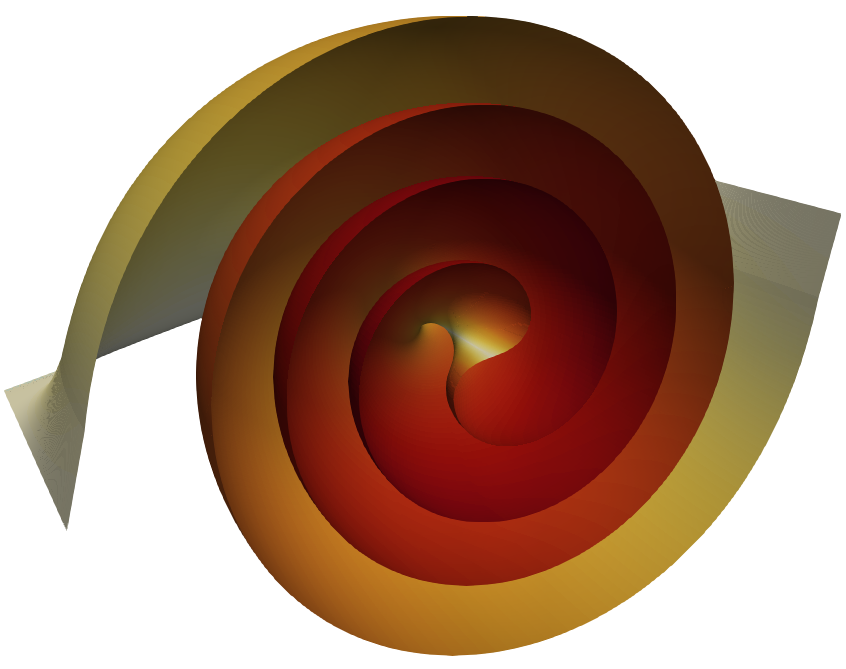
\includegraphics[width=0.188\figurewidth]{figures/ground_truth_log_highres}%
    };
    \node[anchor=north] at (image1.south) {\small ground truth};

    \node[image, right=of image1] (image2)
    {
        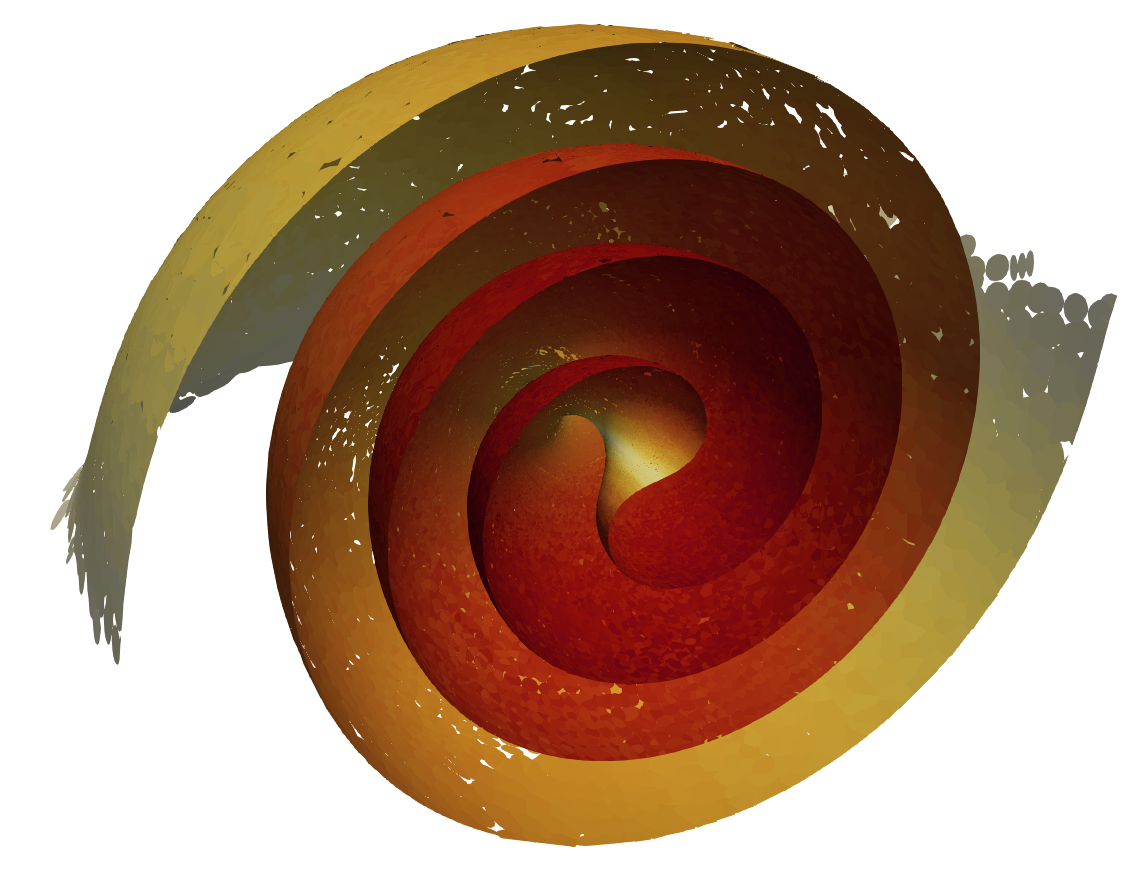
\includegraphics[width=0.188\figurewidth]{figures/norm_0_5_tan_0_01_log}%
    };
    \node[anchor=north, align=left] at (image2.south)
    {
        \small $r_\shortparallel = 0.01$ \\ \small $N = \num{143.5}\si{\kilo}$
    };

    \node[image, right=of image2] (image3)
    {
        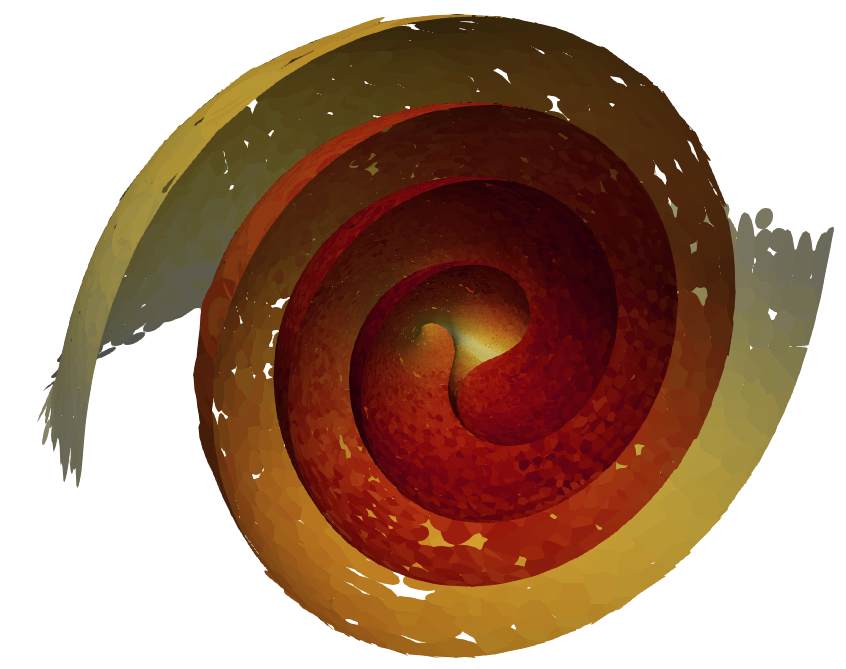
\includegraphics[width=0.188\figurewidth]{figures/norm_0_5_tan_0_02_log}%
    };
    \node[anchor=north, align=left] at (image3.south)
    {
        \small $r_\shortparallel = 0.02$ \\ \small $N = \num{58.1}\si{\kilo}$
    };

    \node[image, right=of image3] (image4)
    {
        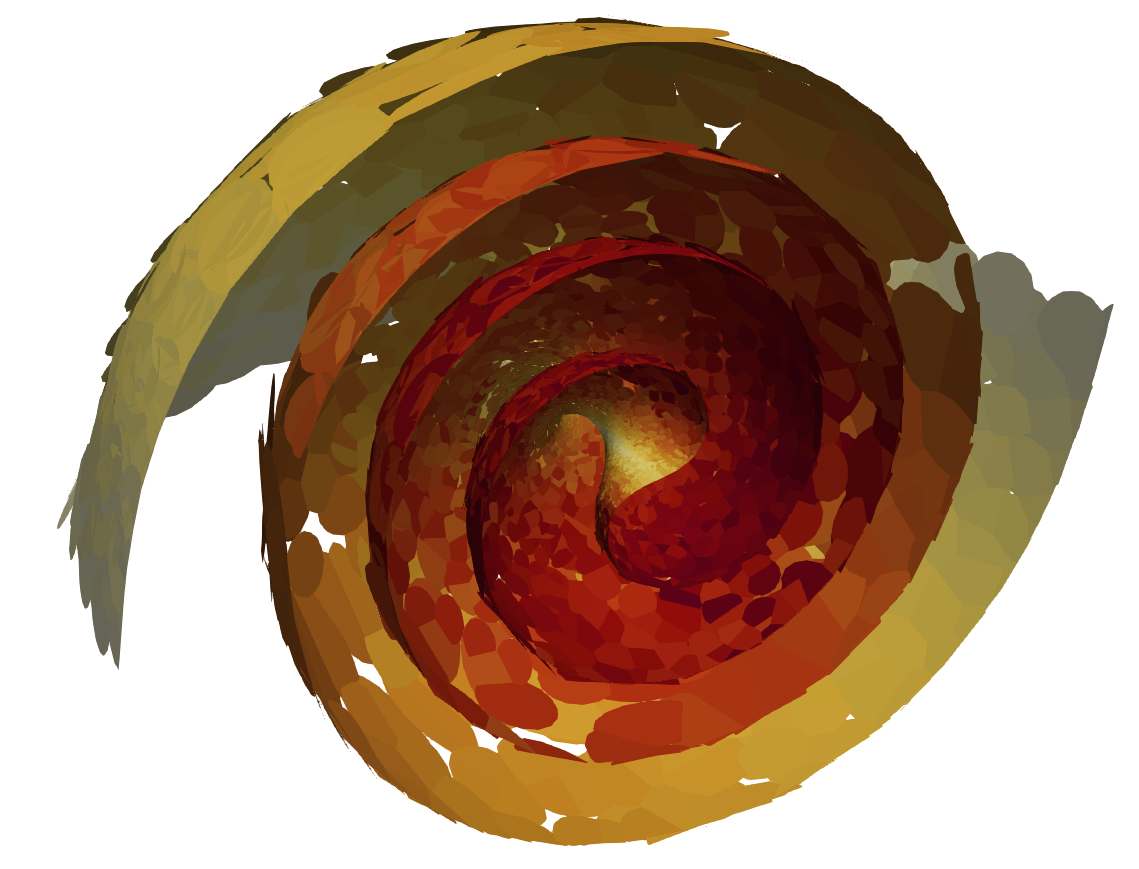
\includegraphics[width=0.188\figurewidth]{figures/norm_0_5_tan_0_05_log}%
    };
    \node[anchor=north, align=left] at (image4.south)
    {
        \small $r_\shortparallel = 0.05$ \\ \small $N = \num{15.4}\si{\kilo}$
    };

    \node[image, right=of image4] (image5)
    {
        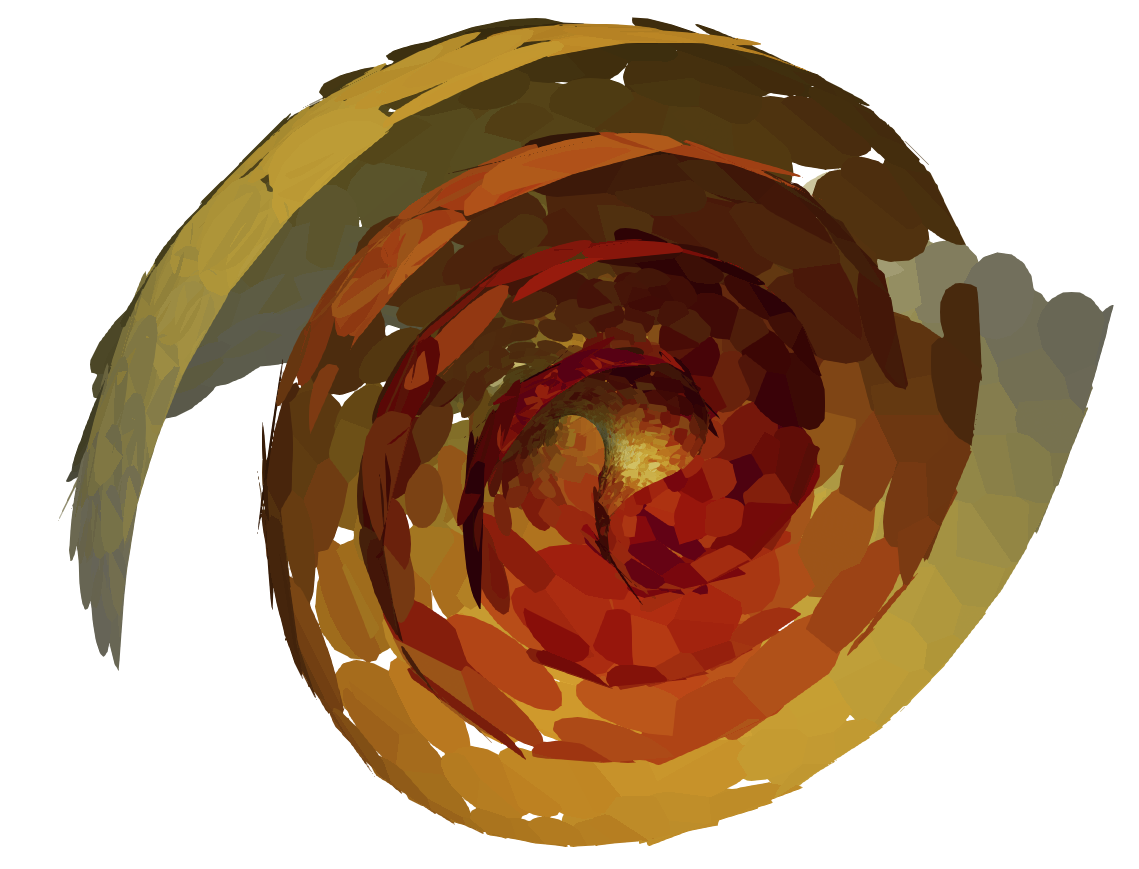
\includegraphics[width=0.188\figurewidth]{figures/norm_0_5_tan_0_1_log}%
    };
    \node[anchor=north, align=left] at (image5.south)
    {
        \small $r_\shortparallel = 0.1$ \\ \small $N = \num{5}\si{\kilo}$
    };

    \node[anchor=west, xshift=-0.5cm] at (image5.east){
        \begin{axis}[
        scale only axis,
        height=2cm,
        hide axis,
        domain=1e0:1e5,
        ymode=log,
        colorbar,
        colorbar/width=0.3cm,
        colormap name={warm},
        point meta min=1e0, point meta max=1e5,
        colorbar style={
            title=$c$,
            scaled ticks=false,
            ytick={1e0, 1e5},
            yticklabels = {$10^{\,0}$, $10^{\,5}$}
        }]
      \end{axis}
    };

\end{tikzpicture}